\chapter{Univ Calif - Digitized by Microgoft ® ree}

Music Librurj

It is gratifying to acknowledge Major Gilbert Thompson, Washington, D. C., and Mr. Frank Spalding, Township Principal, Griffith, Indiana, as persons giving valuable aid in making this book presentable. FREDERICK CASTLE.

\begin{figure}[h!]
\centering
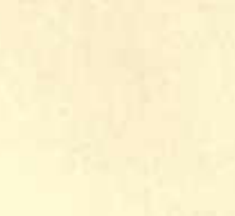
\includegraphics[width=0.8\textwidth]{../imagenes/pagina_012_fig_01.png}
\caption{Figura de la página 12}
\end{figure}

\begin{figure}[h!]
\centering
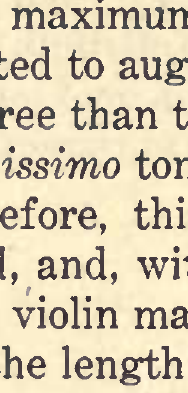
\includegraphics[width=0.8\textwidth]{../imagenes/pagina_012_fig_02.png}
\caption{Figura de la página 12}
\end{figure}

EXPLANATION OF CHART: Because different samples of sounding-board wood must receive different treatment concerning graduation, therefore values for thicknesses are not given; but in lieu of figures, shading is employ- ed as the means of indicating relative quantitive val- ues. The single experiment noted in the text, and, having maximum evenness of tone-power in view, operated to augment altissimo tones in a more marked degree than tones of lower pitch. Because power in altissimo tones is desirable and difficult to secure, therefore, this method for graduation is given record, and, with the hope that future stu- dents of the violin may continue the experiment of shortening the length of sounding-board activity to augment tones of higher pitch. Trial will un- doubtedly determine a better ratio than 2-3 for shortening fiber-activity beneath the lighter strings.

\section{VI}

CHART, indicating by shading, the relative quantitive values of violin sounding-board graduation for maximum

\section{evenness of tone-power.}
